\documentclass[11pt,twoside,a4paper,titlepage]{article}
\usepackage[utf8]{inputenc}
\usepackage[english,german]{babel}
\usepackage{utopia}
\usepackage[margin=2cm]{geometry}
\usepackage[parfill]{parskip}
\usepackage{makeidx}
\usepackage[onehalfspacing]{setspace}
\usepackage{fancyhdr}
\usepackage{lastpage}
\usepackage{hyperref}
\usepackage{graphicx}
\renewcommand{\sffamily}{phv}

\newcommand{\titleText}{Experiment\\Berechnung des Luftwiderstands}
\newcommand{\authorText}{N. Meier, P. Günthard\\Berufsbildungsschule Winterthur, 6MT13v}
\newcommand{\dateText}{\today}

\title{\titleText}
\author{\authorText}
\date{\dateText}

\pagestyle{fancy}
\fancyhf{}

\fancyhead[EL]{\titleText}
\fancyhead[OR]{\authorText}
\cfoot{\thepage \space von \pageref{LastPage}}

\begin{document}
	\maketitle
	\tableofcontents

    \section{Einleitung}
    
   	Dieses Experiment wurde im Rahmen des Physikunterichts der Klasse 6MT13v der BBW durchgeführt. Begleitende Lehrperson war X. Würms.
    
    \section{Beschreibung des Experiments}

	Das Experiment dient dazu, die physikalischen Gesetze des Luftwiderstand zu erarbeiten und zu erlernen. 

\subsection{Aufbau des Experiments}

Für das Experiment wurden folgende Mittel verwendet:

\begin{itemize}
	\item Enfernungsmesser
	\item Testobjekte in Form von Papierkegel
\end{itemize}

Diese wurden wie in der Abbildung \ref{fig:expsetup} angeordnet.

\begin{figure}
	\center
	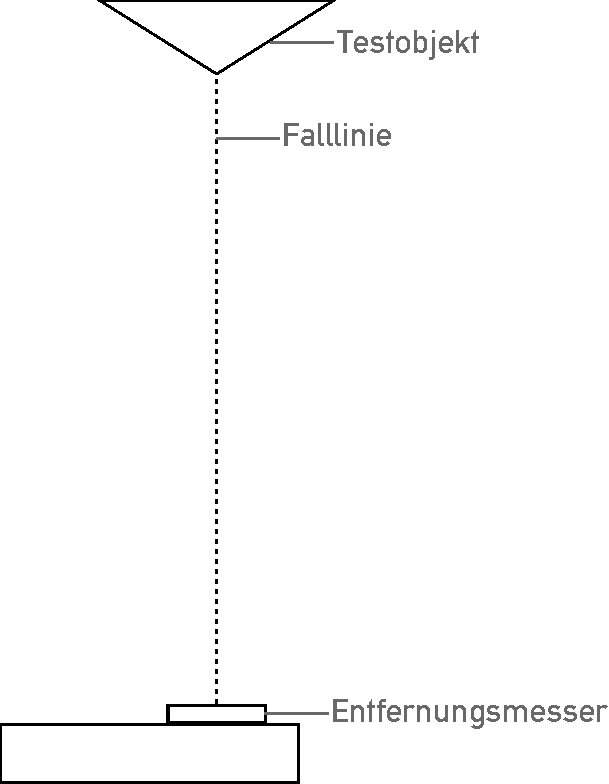
\includegraphics[width=5cm]{diagrams/experiment_aufbau}\caption{\label{fig:expsetup} Aufbau des Experiments}	
\end{figure}

    
    \section{Auswertung}

	\begin{tabular}{|l|l|}
	\hline
	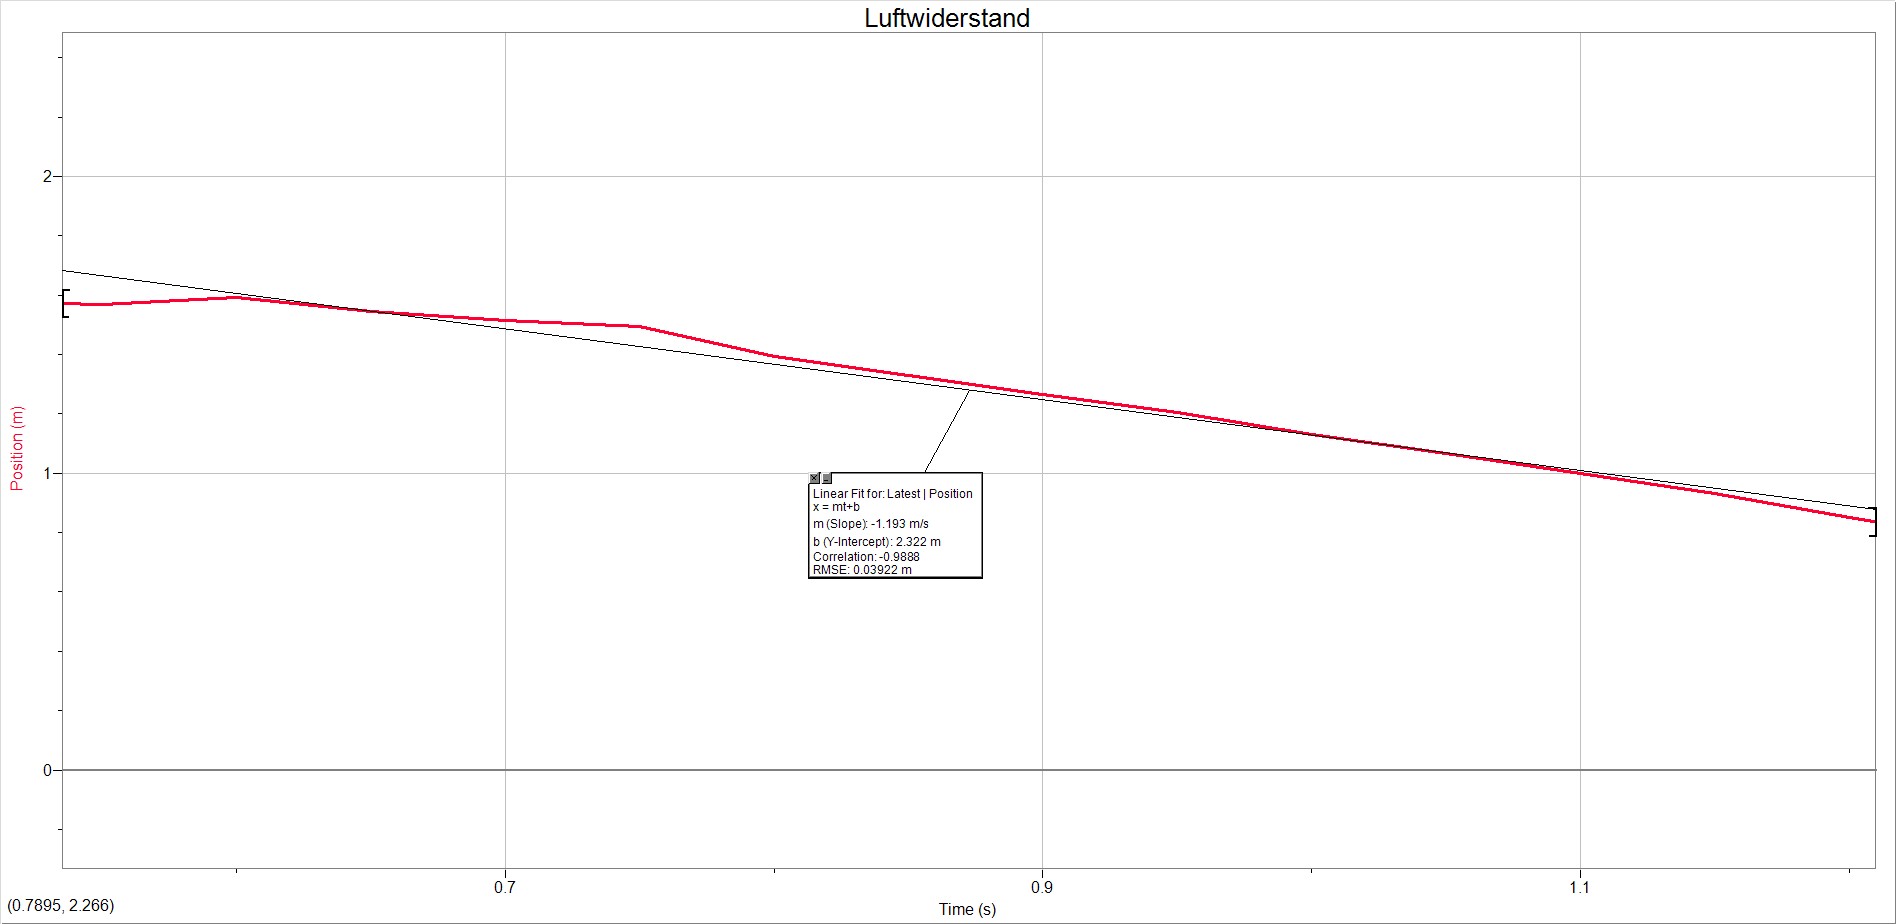
\includegraphics[width=8cm]{graphs/scr1} &
	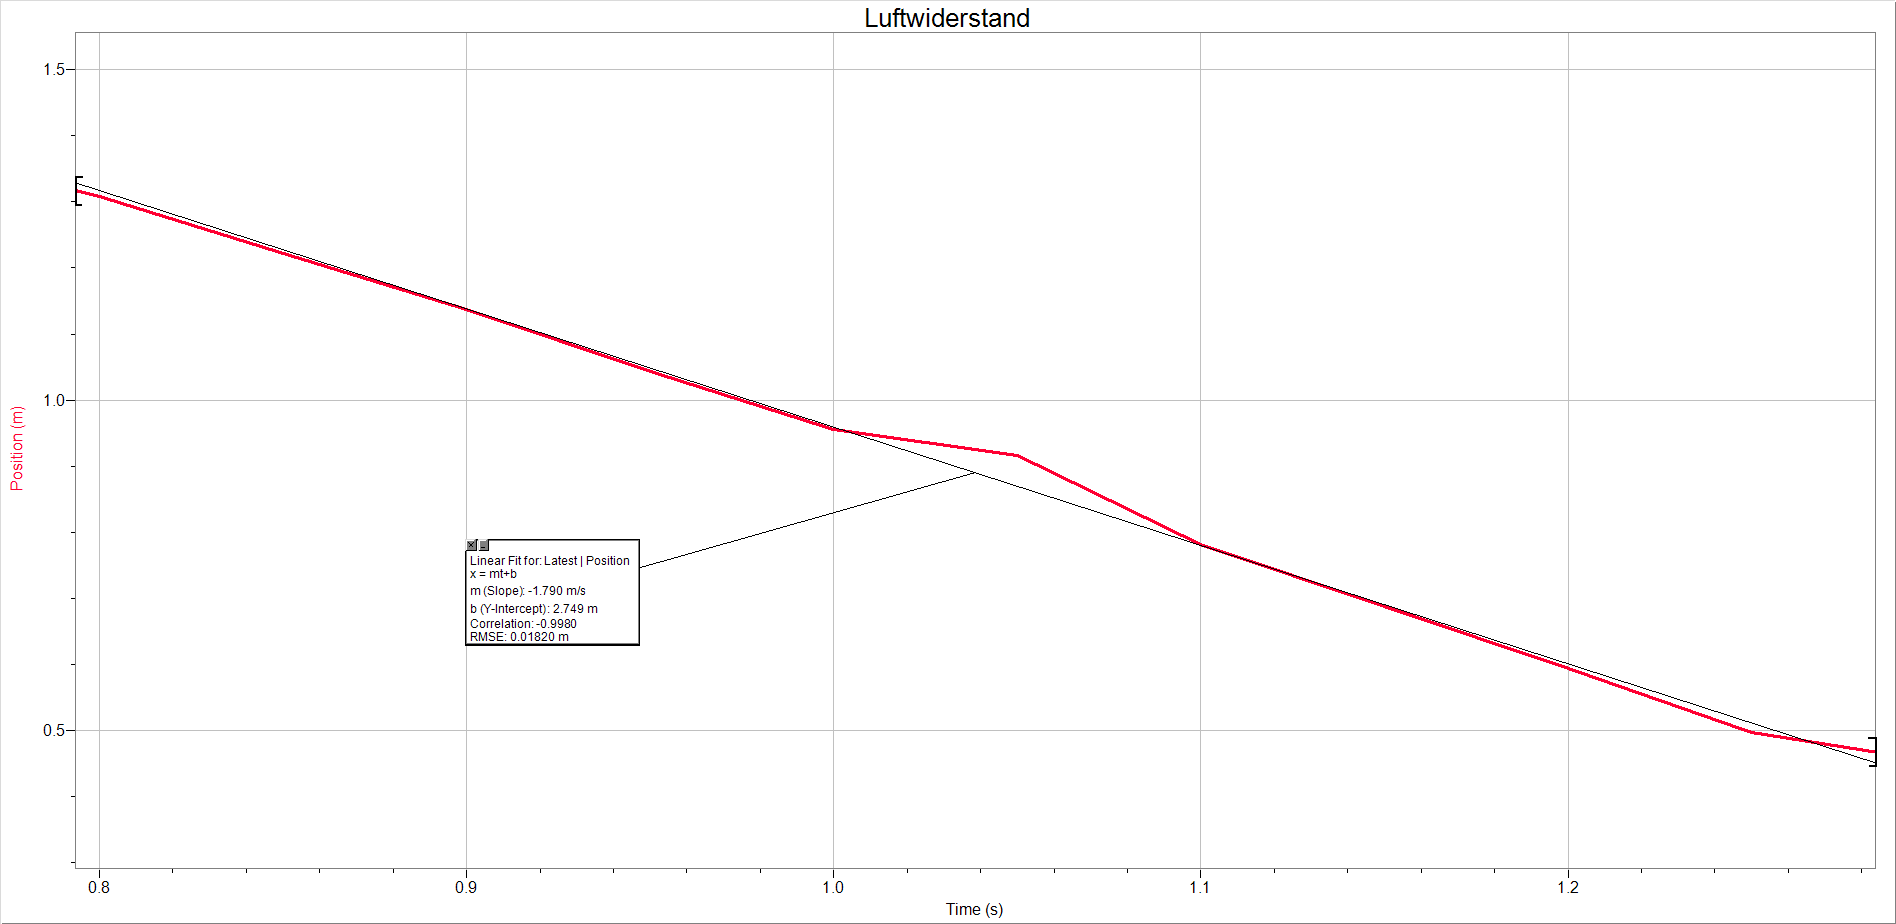
\includegraphics[width=8cm]{graphs/scr2}
	\\\hline 
	1 Kegel: \(-1.193 \frac{m}{s} \) &
	2 Kegel: \(-1.790 \frac{m}{s}\)
	\\\hline
	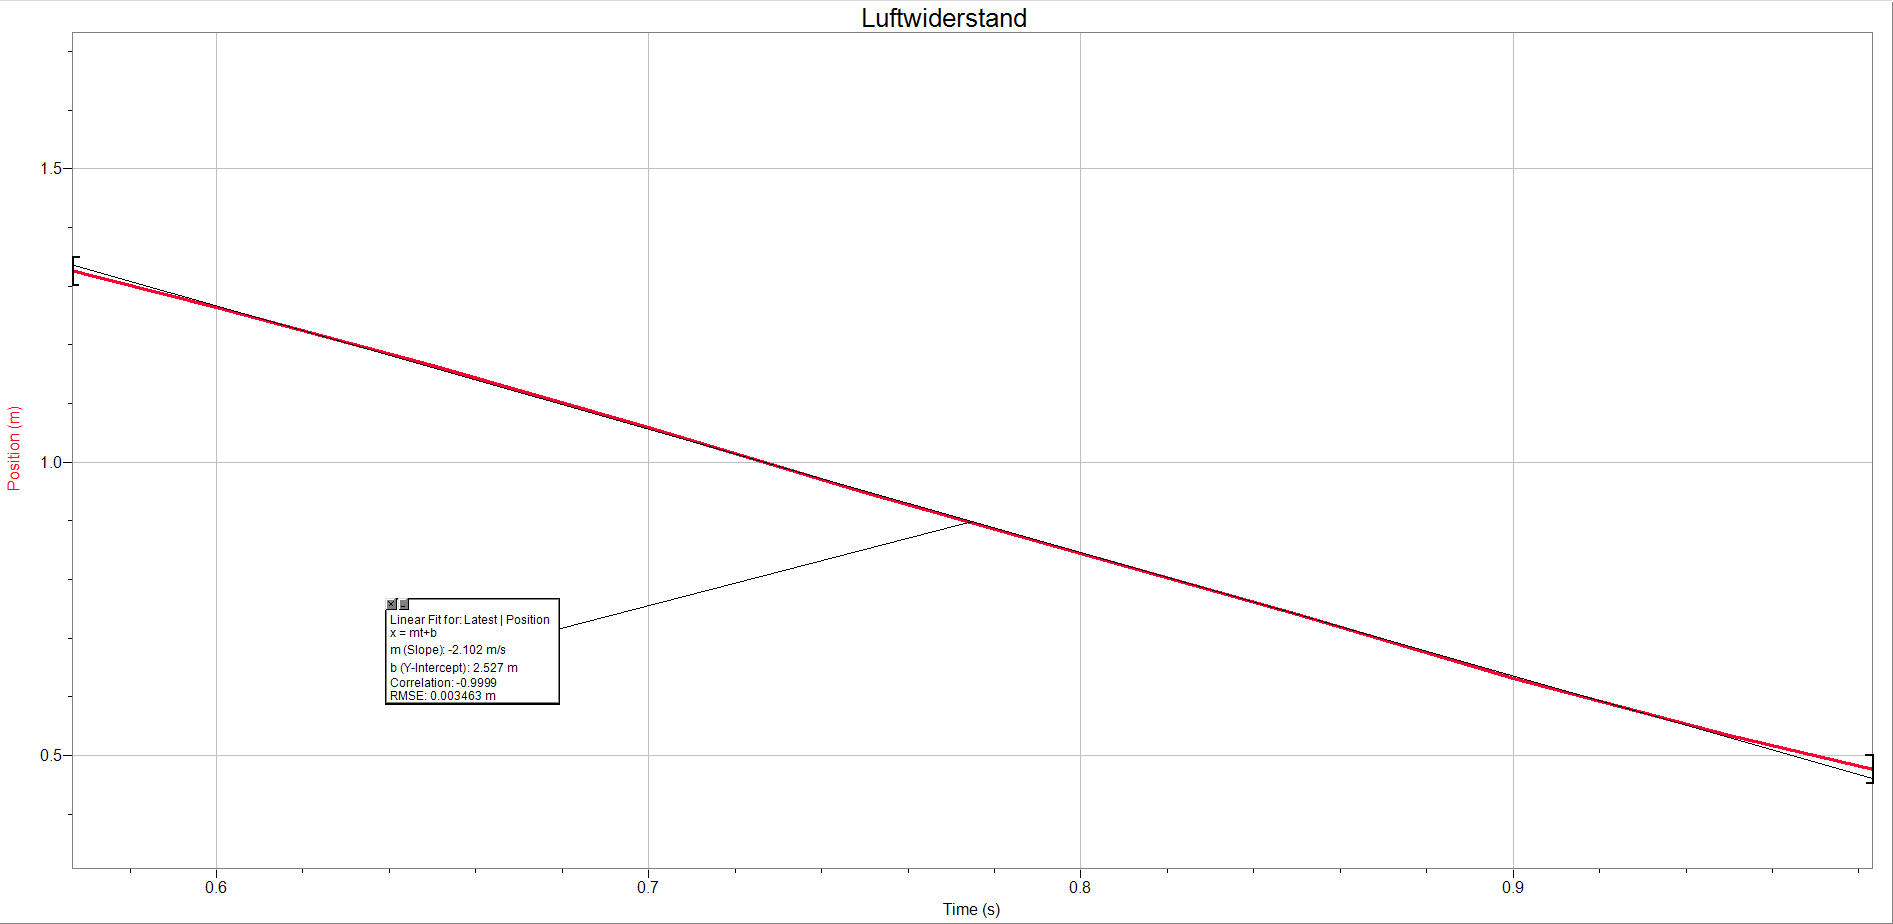
\includegraphics[width=8cm]{graphs/scr3} &
	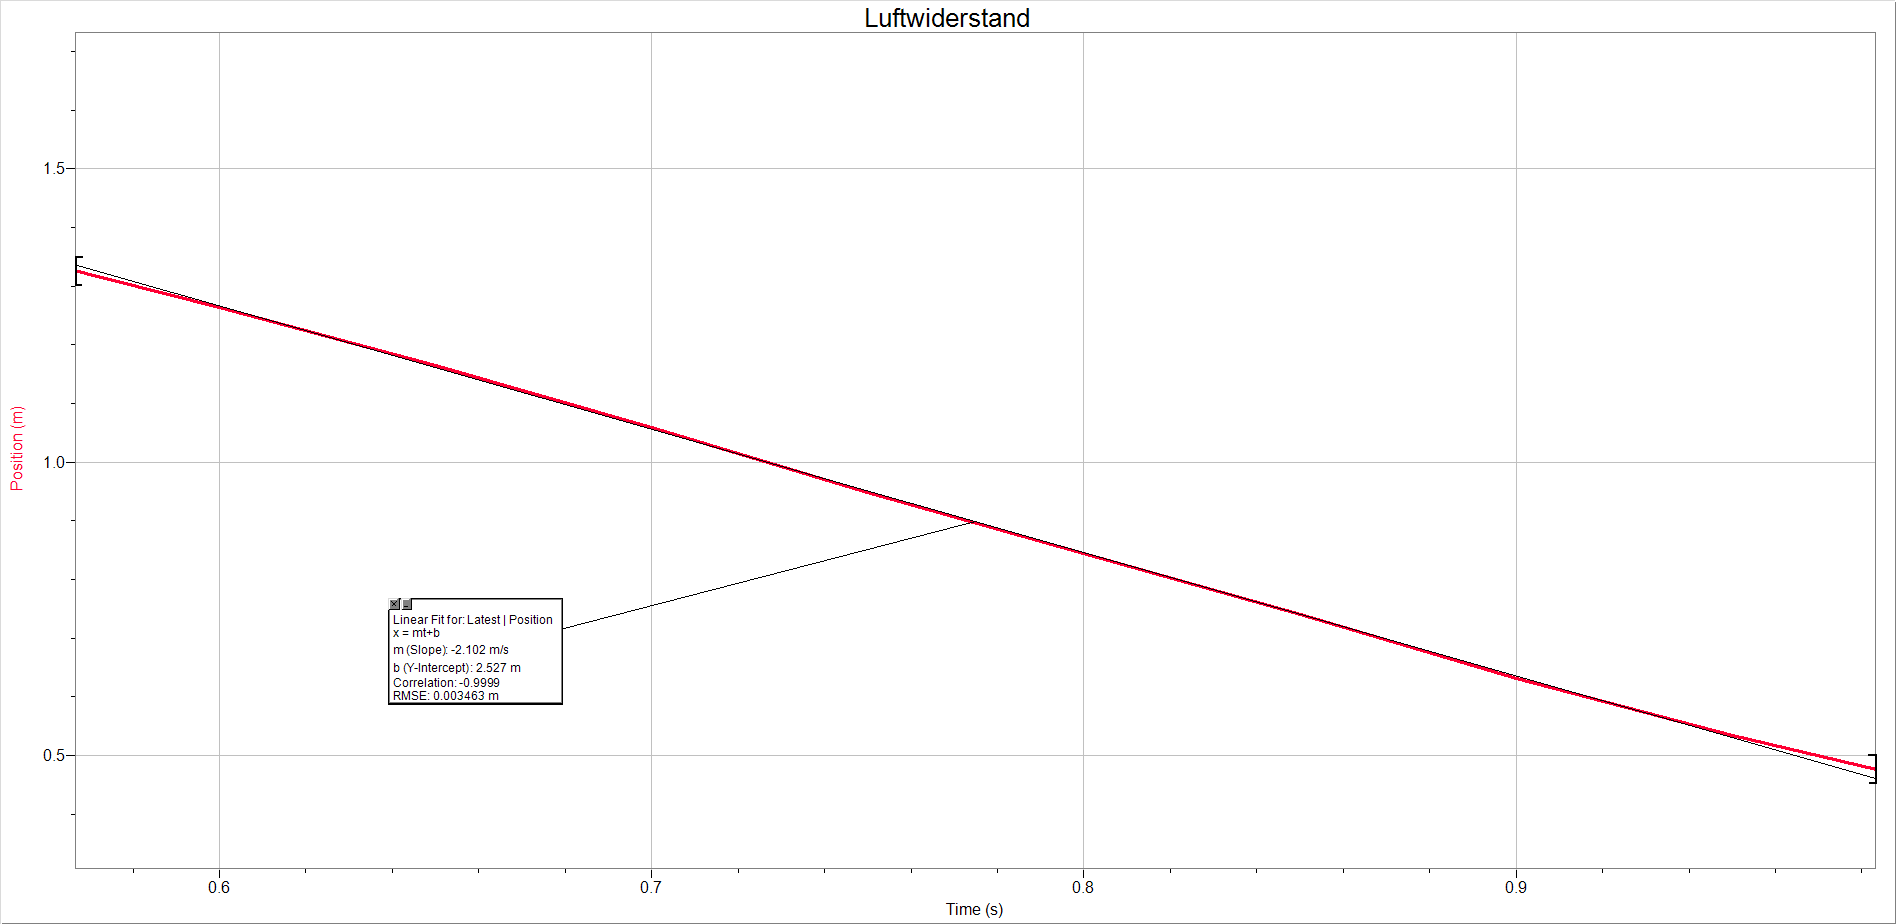
\includegraphics[width=8cm]{graphs/scr4}
	\\\hline 
	3 Kegel: \(-2.102\frac{m}{s} \) &
	4 Kegel: \(-2.547\frac{m}{s}\)
	\\\hline
	
\end{tabular}
    
    \section{Analyse}

	Die Auswertung der Resultate zeigt mehrere Punkte. Es zeigt, dass die erreichte Geschwindigkeit zwar vom Gewicht des Testobjekts abhängt

    \section{Formeln}
	
	\begin{multicols}{2}
	

\(v^2 \sim m \sim F_L\)

\subsection{Laminar}

\(F_L = k * v\)

\subsection{Turbulenzen}

\(F_T = k * v^2 \)

\subsection{Grafische Darstellung}

\textit{Siehe Abbildung \ref{fig:tablegraph}}

\begin{figure}
	\centering
	\begin{tabular}{|l|l|l|}
		\hline
		\textbf{v} & \textbf{\(F\) Laminar} & \textbf{\(F\) Turbulent} \\
		\hline
		0 & 0 & 0\\ \hline
		1 & 1 & 1\\ \hline
		2 & 2 & 4\\ \hline
		3 & 3 & 9\\ \hline
		4 & 4 & 16\\ \hline
		5 & 5 & 25\\ \hline
		
	\end{tabular}
	\caption{\label{fig:tablegraph}}
\end{figure}

\end{multicols}

    
    \section{Schlussfolgerung \& Fazit}
    
\end{document}
